\section{DPG for convection-diffusion}

The convection-diffusion problem can be given as a first order system: 
\begin{align*}
\div \left(\beta u - \sigma\right) &= f\\
\frac{1}{\epsilon}\sigma - \grad u &= 0,
\end{align*}
with inflow boundary conditions $\left.u\right|_{\Gamma_{\rm in}} = u_{\rm in}$, and outflow boundary conditions $\left.u\right|_{\Gamma_{\rm out}} = u_{\rm out}$.  The inflow and outflow boundaries are defined
\begin{align*}
\Gamma_{\rm in} &\coloneqq \{x\in \Gamma; \beta_n(x) \leq 0\}, \quad {\rm (inflow)}\\ 
\Gamma_{\rm out} &\coloneqq \{x\in \Gamma; \beta_n(x) > 0\}, \quad {\rm (outflow)}
%\Gamma_{0} &\coloneqq \{x\in \Gamma; \beta_n(x) = 0\},
\end{align*}
On domain $\Omega$, with mesh $\Oh$ and mesh skeleton $\Gh$, the ultra-weak variational formulation for convection-diffusion is
\begin{align*}
b\left(\left(u,\sigma, \widehat{u}, \widehat{f}_n\right),\left( v, \tau \right)\right) &= 
\left(u,\div \tau - \beta \cdot \grad v\right)_{\Oh} + \left(\sigma, \epsilon^{-1} \tau + \grad v\right)_{\Oh} 
- \LRa{\jump{\tau\cdot n}, \widehat{u} }_{\Gh} + \LRa{ \widehat{f}_n, \jump{v} }_{\Gh}.
\end{align*}
with $v\in H^1$ and $\tau \in H({\rm div},\Oh)$. 

\subsection{Inflow boundary condition and choice of test norm}
\seclab{sec:testNormSec}

Given the above properties of DPG, we can see that the choice of test norm will determine the behavior of DPG; however, the proper choice of test norm can be unclear.  There exists a canonical graph norm for the ultra-weak variational formulation under which well-posedness can be proven for a large class of problems, and near-optimality is observed in numerical experiments \cite{DPG4, Bui-ThanhDemkowiczGhattas11b, stokesDPG}.  However, for the specific problem of convection-diffusion, the resolution of optimal test functions resulting from the graph norm prove very difficult to approximate \cite{globalLocalDPG}.  In \cite{DPGrobustness}, Demkowicz and Heuer introduced guidelines for the construction of alternative test norms based on energy estimates for the adjoint equation. We follow \cite{DPGrobustness2}, where, in addition to constructing an alternative test norm, a new inflow boundary condition is introduced in order to regularize the adjoint equation.  

Typical boundary conditions for the convection-diffusion problem enforce a Dirichlet condition on both inflow and outflow.  We adopt instead a``conserved flux'' inflow boundary condition, 
\[
\beta_nu - \epsilon\pd{u}{n} \approx u_{\rm in}.
\]
This corresponds to the imposition of a boundary condition on the conserved flux $\fnh = \beta_nu - \sigma_n$.  For small $\epsilon$ and most problems of interest, both $\pd{u}{n}$ and $\epsilon$ tend to be small, such that the above is a good approximation of $\left.u\right|_{\Gamma_{\rm in}} = u_{\rm in}$.

Under this boundary condition, the adjoint problem is regularized such that its solutions are smoother, which in turn improves the stability of the DPG method \cite{DPGrobustness2}.  We illustrate this improvement with a simple numerical experiment; Figure~\ref{fig:confusion1D} demonstrates the behavior of the DPG method under both the standard Dirichlet and the new conserved flux boundary conditions.  In both cases, the test norm used is the 1D Sobolev norm $\nor{\LRp{v,\tau}}_V\coloneqq \nor{v}_{H^1} + \nor{\tau}_{H^1}$.  The left figure shows the behavior of DPG under a Dirichlet boundary condition; degeneration of the solution is observed as $\epsilon$ decreases.  In contrast, under the new conserved flux boundary condition, as $\epsilon$ decreases, the solution converges to the $L^2$ projection of the exact solution onto our trial space.  

\begin{figure}
\centering
\subfigure[Dirichlet boundary condition $u(0) = 1$]{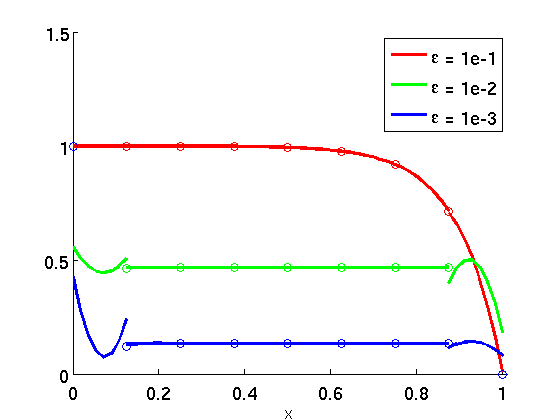
\includegraphics[width=2.75in]{dirichletBC.png}}
\subfigure[``Conserved flux'' boundary condition $u(0) - \epsilon u'(0) = 1$]{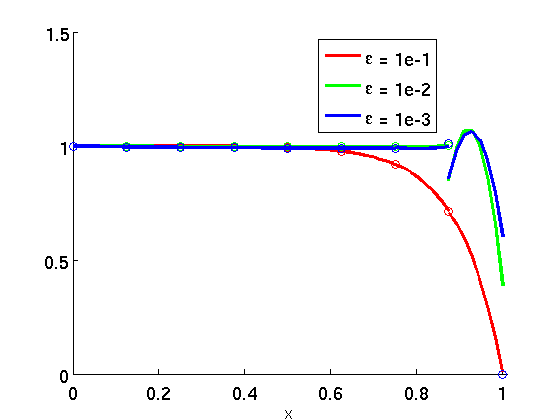
\includegraphics[width=2.75in]{newBC.png}}
\caption{Behavior of the 1D DPG method for convection diffusion under both standard Dirichlet and conserved flux boundary conditions.}
\label{fig:confusion1D}
\end{figure}

The test norm for convection-diffusion in multiple dimensions is defined elementwise on $K$ as
\[
\|\left(v,\tau\right)\|_{V,K}^2 = \min\left\{\frac{\epsilon}{|K|},1\right\}\|v\|^2 + \epsilon \|\grad v\|^2 + \|\beta \cdot \grad v\|^2 + \| \div \tau-\beta\cdot\grad v\|^2 + \min\left\{\frac{1}{\epsilon},\frac{1}{|K|}\right\}\|\tau\|^2.
\]
DPG under $\nor{\cdot}_V$ both delivers robust control of the $L^2$ error in the variables $u$ and $\sigma$ and minimizes approximation error in the solution of \eqnref{optvVar}.

\subsection{Anisotropic refinement}
\seclab{sec:aniso}
Isotropic adaptive mesh refinement has shown itself to be an effective way to resolve isolated solution features with large gradients, such as point singularities \cite{hp1,hp3}. However, for the resolution of phenomena such as shocks or boundary layers, anisotropic mesh refinement can resolve solution features for a much lower cost per degree-of-freedom, due to the fact that boundary layers in $n$-dimensions are primarily phenomena supported over $n-1$ dimensions.  

As a least squares method, DPG already includes a natural error indicator with which to drive adaptive mesh refinement.  To introduce anisotropic refinements, we need to introduce an anisotropy indicator in order to detect in which direction solution features are aligned.  In general, a test norm can be expressed as the sum of normed quantities, both scalar and vector valued.  If we restrict ourselves to quadrilateral elements for the moment, a general anisotropy indicator for DPG can be constructed by evaluating the $\L$ norms of the individual components of vector valued terms in the test norm.  

Under the robust test norm derived in this chapter for the convection-dominated diffusion problem, we can define $x$ and $y$ error contributions over a single element
\begin{align*}
e_{x,K} &= \epsilon \nor{\pd{v}{x}}_{L^2(K)}^2 + \nor{\tau_x}_{L^2(K)}^2 \\
e_{y,K} &= \epsilon \nor{\pd{v}{y}}_{L^2(K)}^2 + \nor{\tau_y}_{L^2(K)}^2.
\end{align*}
We define the anisotropy indicator as the ratio $r_K = \frac{e_{x,K}}{e_{y,K}}$, and implement a simple refinement scheme following \cite{DPG3}.  Given some anisotropic threshold $\epsilon_r$, if $r_K>\epsilon_r$, then we can conclude that the error in the $x$ direction is large compared to the $y$ direction, and we anisotropically refine the element along the $x$-axis.  Likewise, if $r_K < \frac{1}{\epsilon_r}$, this implies that the opposite is true, and we refine the element anisotropically along the $y$-axis.  

%We note that it is possible to compute the discrete system without needing much additional integration.  Recall that if we let $G$ be the symmetric positive-definite Gram matrix representing the inner product $\LRp{v,\delta v}_V$ on $V_h$, we solve for degrees of freedom $c_e$ representing our error representation function $e$.  
%
%For both the graph and robust test norms, we can decompose the inner product that induces the test norm into 
%\[
%\LRp{v,\delta v}_V = \sum_i \LRp{v,\delta v}_{V,x_i} + \LRp{v,\delta v}_{V,{\rm scalar}}
%\]
%such that $\LRp{v,\delta v}_{V,x_i}$ is a seminorm containing the $i$th coordinate component of a vector-valued test term, and $\LRp{v,\delta v}_{V,{\rm scalar}}$ is simply the non-vector portions of the test norm.  For example, if we take the $H^1(\Omega)$ Sobolev norm
%\[
%\LRp{v,\delta v}_V = \LRp{v,\delta v}_{\L} + \LRp{\grad v,\grad \delta v}_{\L}
%\]
%then $\LRp{v,\delta v}_{V,x_i} = \LRp{\pd{v}{x_i},\pd{\delta v}{x_i}}_{\L}$, and $\LRp{v,\delta v}_{V,{\rm scalar}} = \LRp{v,\delta v}_{\L}$.  Each bilinear term $\LRp{v,\delta v}_{V,x_i}$ induces a symmetric positive-semidefinite matrix $G_{x_i}$, such that 
%\[
%c_e^TG_{x_i}c_e = \nor{e}^2_{V,x_i}.
%\]
%By storing $G$ as the sum of $G_{\rm scalar}$ and $G_{x_i}$, we can then cheaply compute the anisotropic error indicators once we have the degrees of freedom corresponding to our error representation function.  

